%\documentclass[a4paper,10pt]{article}
\documentclass[a4paper,10pt]{scrartcl}
\usepackage[margin=0.5in]{geometry}

\usepackage[utf8]{inputenc}

\usepackage{wrapfig}
\usepackage{lscape}
\usepackage{rotating}

\usepackage{amssymb}
\usepackage{hyperref}
\usepackage[square]{natbib}

%fancy stuff
%\usepackage{datetime}
\usepackage{helvet,mathptmx}
\usepackage{xcolor}
\usepackage[normalem]{ulem} % striked-out text

\usepackage{verbatim}
%\usepackage{listings}

\usepackage{graphicx} %, subfigure
\usepackage{caption}
% %\usepackage{subcaption} incompatible with some templates, so use subfig instead
\usepackage[caption=false]{subfig}
\usepackage{float}
\usepackage{wrapfig}
\usepackage{placeins}

\title{Bayesian MMM example}
\author{Onur Kerimoglu}
%\date{\today}
\date{03.02.2023}

\pdfinfo{%
  /Title    (Bayesian MMM)
  /Author   (Onur Kerimoglu)
  /Creator  (Onur Kerimoglu)
  /Producer ()
  /Subject  ()
  /Keywords ()
}


\graphicspath{
{.}
}

\begin{document}


\maketitle

\section{Background}
In a nutshell, the task is in the context of performance marketing and the task is to apply a bayesian mixed-media model (MMM) on our test dataset an interpret the insights from the model.

The sourcode of the notebook with which the presented material is produced, and this report itself is publicly available \href{https://github.com/OnurKerimoglu/bayesian_mmm/examples/bayesian_mmm_example_enhanced_newdataset.ipynb}{here}.

\section{Answers}

\subsection{How do you model spend carry over?}

To describe carryover, I used a simple geometric decay function as in \href{https://static.googleusercontent.com/media/research.google.com/en//pubs/archive/46001.pdf}{Jin et al. (2017)}:

\begin{equation}\label{eq:carryover}
 w_i = \alpha_i^l, l=0,...,L-1, 0<\alpha_i<1
\end{equation}

where $w_i$ describes the weight of the effect on   $\alpha_i$ is the decay rate for channel $i$. Here, I assumed the max. duration ($L$) to be 14 days, which, might be possible to fit to data as well.

\subsection {Explain your choice of prior inputs to the model?}

Here is the procedure I followed:
\begin{itemize}
 \item In order to ensure positive coefficients I draw the coefficient spendings from a Half-Normal distribution.
 \item I referred to earlier work, such as Jin et al. (2017) to choose the distributions and limits, such as drawing $\alpha_i$ in Eq.~\ref{eq:carryover} from a beta distribution, and earlir examples, such as \href{https://towardsdatascience.com/bayesian-marketing-mix-modeling-in-python-via-pymc3-7b2071f6001a}{the blogpost by Robert Kübler} and \href{https://towardsdatascience.com/modeling-marketing-mix-using-pymc3-ba18dd9e6e68}{another one by Slava Kisilevich}.
 \item I adjusted the priors slightly until obtaining some overlap between the observed revenue and model results based on prior sampling (Fig.~\ref{f:pred_prior}).
\end{itemize}

 
\begin{figure}[!h]
  \centering
  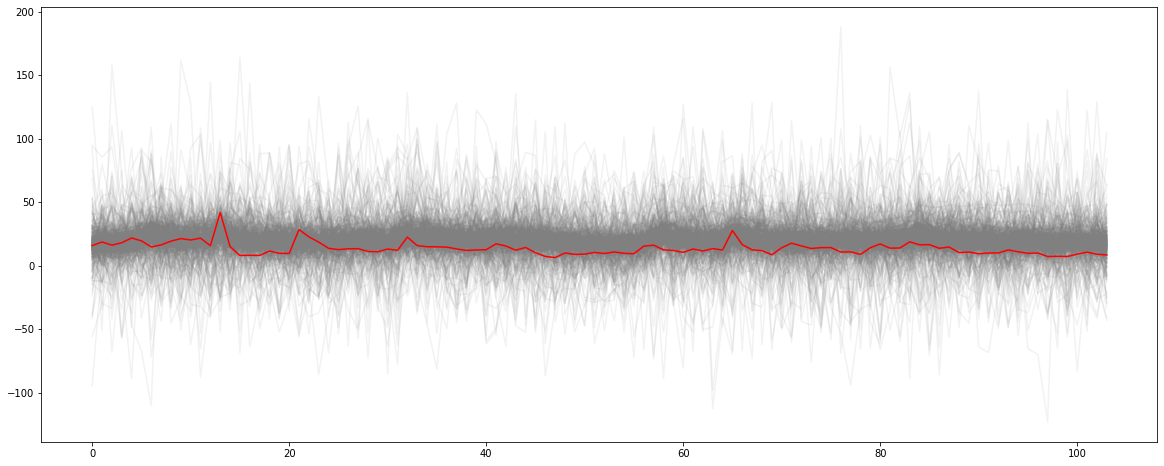
\includegraphics[trim=0mm 0mm 0mm 0mm, clip, width=.8\textwidth]{Prior_prediction.png}
  \caption{Model results based on prior sampling vs scaled (1/10000) observed revenue.}\label{f:pred_prior}
\end{figure}

\FloatBarrier

\subsection {How are your model results based on prior sampling vs. posterior sampling?}
I am not sure if I understand this question well. Fig.~\ref{f:pred_prior} shows the prior predictions of the model vs the observations, where the model doesn't show skill, as expected, whereas Fig.~\ref{f:preds_vs_obs} shows that the model based on posterior sampling captures the observed patterns pretty well.

\subsection {How good is your model performing? How you do measure it?}

Predicted vs observed revenue is shown in Fig.~\ref{f:preds_vs_obs}. Except for two weeks, the observations lay within 2 standard deviations plus/minus the predictions. That instance is likely due to a special event, like a promotion or a holiday, which is not accounted for by the model. The mean absolute error is 26938 EUR (?), which corresponds to about 20\% in terms of percentage. 

\begin{figure}[!h]
  \centering
  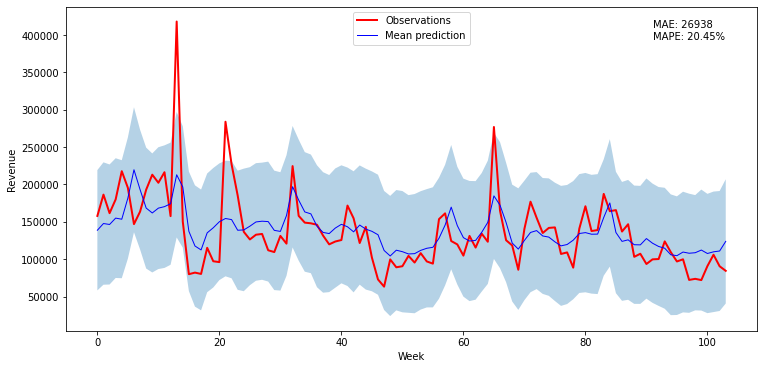
\includegraphics[trim=0mm 0mm 0mm 0mm, clip, width=.8\textwidth]{preds_vs_obs.png}
  \caption{Predicted ($\pm 2\sigma$) vs observed revenue.}\label{f:preds_vs_obs}
\end{figure}


\FloatBarrier

\subsection {(Bonus) Can you derive ROI (return on investment) estimates per channel? What is the best channel in terms of ROI?}
Results are shown in Fig.~\ref{f:CS_ROI}. For each channel $i$, percentage $ROI^i$ was calculated according to:
\begin{equation}\label{eq:roi}
 ROI^i = \frac{\sum_t C_t^i - \sum_t S_t^i}{\sum_t S_t^i} * 100
\end{equation}
where $C_t^i$ and $S_t^i$ are the revenue contribution and spends to the channel $i$ at a given time ($t$).  


\begin{figure}[!h]
  \centering
  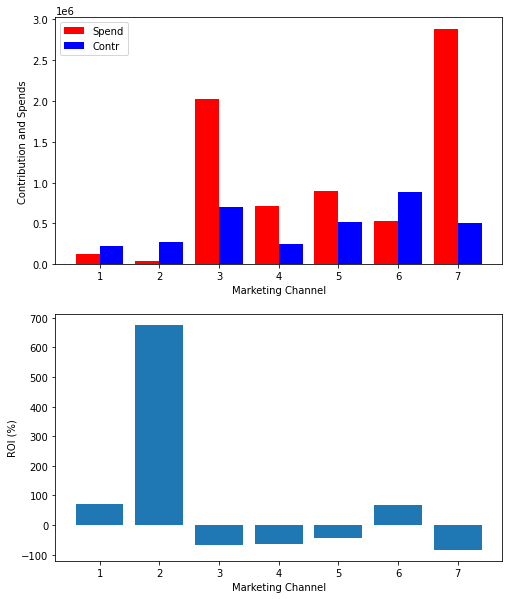
\includegraphics[trim=0mm 0mm 0mm 0mm, clip, width=.5\textwidth]{contributions_roi.png}
  \caption{Top: Total spends ($\sum_t S_t^i$) and revenue contributions ($\sum_t C_t^i$); bottom: ROI (\%) for each channel $i$ (see Eq.~\ref{eq:roi}).}\label{f:CS_ROI}
\end{figure}

\FloatBarrier

\subsection {What are your main insights in terms of channel performance/effects?}


Only channels 1, 2 and 6 seem to generate positive net gains (Fig.\ref{f:CS_ROI}). Among these channels, 2 seems most effective in terms of ROI, however, in terms of absolute revenue contribution, channel 6 is the most important source. Among the channels that results in net costs channel 7 is the one that requires most immediate attenion, both in terms of ROI and absolute net cost. Continued investment in channels 3 and 4 seem also questionable.

It is important to note that, according to the model, a large portion of the revenue is not explained by marketing actions (Fig.\ref{f:Conts}).
\begin{figure}[!h]
  \centering
  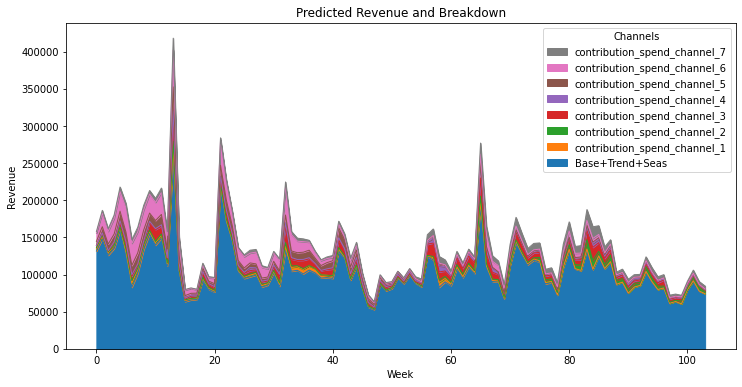
\includegraphics[trim=0mm 0mm 0mm 0mm, clip, width=.8\textwidth]{contributions_vs_time.png}
  \caption{Contributions and baseline (+trend \& seasonality) over time}\label{f:Conts}
\end{figure}

According to the Prophet model with which the time series analysis was performed, there is a negative trend, and a complex seasonal component (Fig.~\ref{f:TrendSeas}). Further work is needed to discover the drivers of these components.

\begin{figure}[!h]
  \centering
  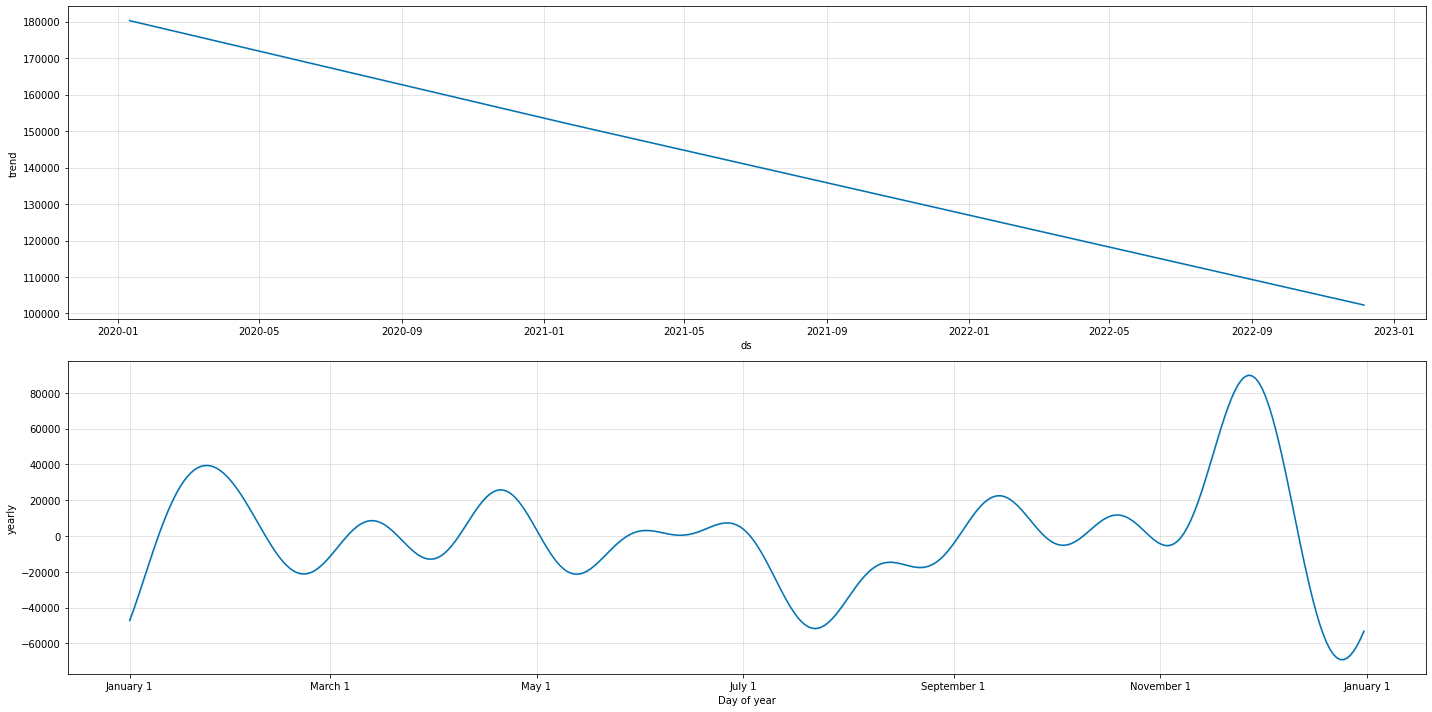
\includegraphics[trim=0mm 0mm 0mm 0mm, clip, width=.8\textwidth]{trend_and_seasonality.png}
  \caption{Trend and seasonal components in revenue}\label{f:TrendSeas}
\end{figure}



%\bibliographystyle{apalike}
%\bibliography{river_report.bib}

\end{document}
